\achapter{6}{Continuous Functions in Metric Spaces}\label{chap:continuous_functions}


\vspace*{-17 pt}
\framebox{
\parbox{\dimexpr\linewidth-3\fboxsep-3\fboxrule}
{\begin{fqs}
\item What does it mean for a function between metric spaces to be continuous at a point?
\item What does it mean for a function between metric spaces to be continuous?
\end{fqs}}}

\vspace*{13 pt}

\csection{Introduction}\label{sec_cont_func_intro}

We have likely had previous experiences with continuous functions. Continuity is an important consideration in optimization problems because a continuous function attains a maximum value and a minimum value on any closed and bounded interval. Continuous functions also satisfy the Intermediate Value Theorem, that a continuous function $f$ takes on all values between $f(a)$ and $f(b)$ on an interval $[a,b]$. An important consequence of the Intermediate Value Theorem is that if $f$ is a continuous function on an interval and $f(a)$ and $f(b)$ have opposite signs, then $f$ must have a root in the interval $[a,b]$. In this section we will begin to explore continuity of functions between metric spaces. Our ultimate goal in future sections is to understand continuous functions well enough that we can define continuity just in terms of open sets. 

In calculus we discuss the idea of continuity. A function $f:\R \to \R$ (using the standard Euclidean metric) is continuous at a point $a$ if 
\[\lim_{x \to a} f(x) = f(a).\]
This involved providing some explanation about what it means for a function $f$ to have a limit at a point. Intuitively, the idea is that a function $f$ has a limit $L$ at $x=a$ if we can make all of the value of $f(x)$ as close to $L$ as we want by choosing $x$ as close to (but not equal to) $a$ as we need. To extend this informal notion of limit to continuity at a point we would say that a function $f$ is continuous at a point $a$ if if we can make all of the value of $f(x)$ as close to $f(a)$ as we want by choosing $x$ as close to $a$ as we need (now $x$ can equal $a$). 

In order to define continuity in a more general context (in topological spaces) we will need to have a rigorous definition of continuity to work with. We will begin by discussing continuous functions from $\R$ to $\R$, and build from that to continuous functions in metric spaces. These ideas will allow us to ultimately define continuous functions in topological spaces. 

We begin by working with continuous functions from $\R$ to $\R$. Our goal is to make more rigorous our informal definition of continuity at a point. To do so will require us to formally defining what we mean by 
\begin{itemize}
\item making the values of $f(x)$ ``as close to $f(a)$ as we want", and
\item choosing $x$ ``as close to $a$ as we need".
\end{itemize}

\begin{figure}[ht]
\begin{center}
\resizebox{!}{2.0in}{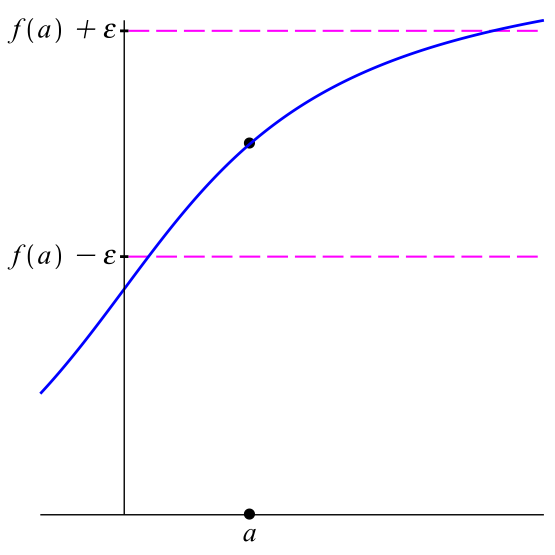
\includegraphics{Continuity_1}} \hspace{0.75in} \resizebox{!}{2.0in}{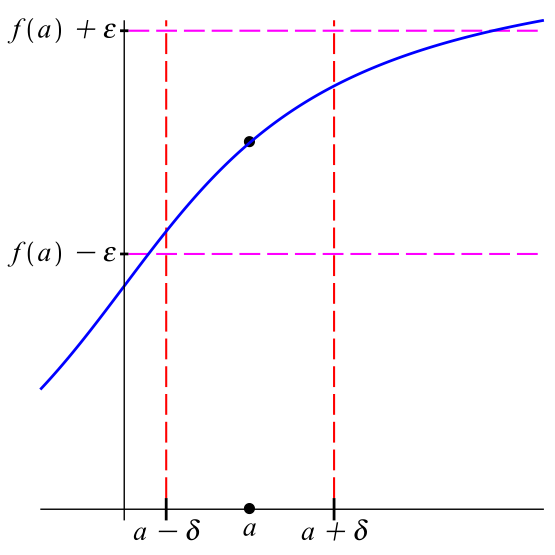
\includegraphics{Continuity_2}}
\caption{Demonstrating the definition of continuity at a point.}
\label{F:Continuity}
\end{center}
\end{figure}
Let's deal with the first statement, making the values of $f(x)$ ``as close to $f(a)$ as we want". What this means is that if we set any tolerance, say $0.0001$, then we can make the values of $f(x)$ within $0.0001$ of $f(a)$. Since the absolute value $| f(x)-f(a) |$ measures how close $f(x)$ is to $f(a)$, we can rewrite the statement that the values of $f(x)$ are within $0.0001$ of $f(a)$ as $| f(x) - f(a) | < 0.0001$. Of course, $0.0001$ may not be as close as we want to $f(a)$, so we need a way to indicate that we can make the values of $f(x)$ arbitrarily close to $f(a)$ -- within any tolerance at all. We do this by making the tolerance a parameter, $\epsilon$. Then our job is to make the values of $f(x)$ within $\epsilon$ of $f(a)$ regardless of the size of $\epsilon$. We write this as 
\[| f(x) - f(a) | < \epsilon.\]
We can picture this as shown at left in Figure \ref{F:Continuity}. Here we want to make the values of $f(x)$ lie within an $\epsilon$ band of $f(a)$ above and below $f(a)$. That is, we want to be able to make the values of $f(x)$ lie between $f(a)-\epsilon$ and $f(a)+\epsilon$. 

Now we have to address the question of how we ``make" the values of $f(x)$ to be within $\epsilon$ of $f(a)$. Since the values $f(x)$ are the dependent values, dependent on $x$, we ``make" the values of $f(x)$ have the property we want by choosing the inputs $x$ appropriately.  In order for $f$ to be continuous at $x=a$, we must be able to find $x$ values close enough to $a$ to force $| f(x) - f(a) | < \epsilon$. Pictorially, we can see how this might happen in the image at right in Figure \ref{F:Continuity}. We need to be able to find an interval around $x=a$ so that the graph of $f(x)$ lies in the $\epsilon$ band around $f(a)$ for values of $x$ in that interval. In other words, we need to be able to find some positive number $\delta$ so that if $x$ is in the interval $(a-\delta, a+\delta)$, then the graph of $f(x)$ lies in the $\epsilon$ band around $y=f(a)$. More formally, if we are given any positive tolerance $\epsilon$, we must be able to find a positive number $\delta$ so that if $| x-a | < \delta$ (that is, $x$ is in the interval $(a-\delta, a+\delta)$), then $| f(x) - f(a) | < \epsilon$ (or $f(x)$ lies in the $\epsilon$ band around $y=f(a)$).   

This gives us a rigorous definition of what it means for a function $f: \R \to \R$ to be continuous at a point.

\begin{definition} \label{def:epsilon_delta_continuity} A function $f : \R \to \R$ is \textbf{continuous at a point} $a$ if, given any $\epsilon > 0$, there exists a $\delta > 0$ so that $| x - a | < \delta$ implies $| f(x) - f(a)| < \epsilon$.
\end{definition}

Note that the value of $\delta$ can depend on the value of $a$ and on $\epsilon$, but not on values of $x$. 

\begin{pa} \label{pa:MS_continuity} The GeoGebra file at \url{https://www.geogebra.org/m/rym36sqs} will allow us to play around with this definition. Use this GeoGebra applet for the first two problems in this activity. 
\be
\item Enter $f(x)=x\sin(x)$ as your function. (You can change the viewing window coordinates, the base point $a$, and the function using the input boxes at the left on the screen.) Determine a value of $\delta$ so that $| f(x) - f(1) | < 0.5$ whenever $| x - 1 | < \delta$. Explain your method.

\item Now find a value of $\delta$ so that $| f(x) - f(2.5) | < 0.25$ whenever $| x - 2.5 | < \delta$. Explain your method.

\item ~
	\ba
	\item What is the negation of the definition of continuity at a point? In other words, what do we need to do to show that a function $f: \R \to \R$ is not continuous at a point $x=a$? 

	\item Use the negation of the definition to explain why the function $f : \R \to \R$ defined by 
	\[f(x) = \begin{cases} -1 &\text{ if } x < 1 \\ 1 &\text{ if } x \geq 1 \end{cases}\]
	is not continuous at $x=1$. 

	\ea
	
\ee


\end{pa}

\begin{comment}

\ActivitySolution
\be
\item We look for a value of $\delta$ so that the graph of $f$ on the interval $(1-\delta, 1+\delta)$ is contained entirely within the band $(f(1)-0.5, f(1)+0.5)$. A value of $\delta$ that works in this case is $\delta = 0.3$, as illustrated at left in Figure \ref{F:PA_Continuity_2}. 
 
\begin{figure}[ht]
\begin{center}
\resizebox{!}{1.8in}{\includegraphics{PAContinuity_a}} \hspace{0.5in} \resizebox{!}{1.8in}{\includegraphics{PAContinuity_b}}
\caption{Continuity at a point for Preview Activity \ref{pa:MS_continuity}.}
\label{F:PA_Continuity_2}
\end{center}
\end{figure}

\item  We look for a value of $\delta$ so that the graph of $f$ on the interval $(2.5-\delta, 2.5+\delta)$ is contained entirely within the band $(f(2.5)-0.25, f(2.5)+0.25)$. A value of $\delta$ that works in this case is $\delta = 0.1$, as illustrated at right in Figure \ref{F:PA_Continuity_2}. 

\item ~
	\ba
	\item  We negate a universal quantifier with an existential quantifier and an existential quantifier with a universal quantifier. So a function $f : \R \to \R$ is not continuous at $x=a$ if there exists an $\epsilon > 0$ so that for all $\delta > 0$, the fact that $| x-a | < \delta$ does not imply $| f(x) - f(a) | < \epsilon$. 

	\item  The graph of $f$ is shown in Figure \ref{F:PA_Continuity_3}. Let $\epsilon = 0.5$. Given $\delta > 0$, the point $x = 1-\frac{\delta}{2}$ is in the interval $(1-\delta, 1+\delta)$, but  
\[| f(x) - f(1) | = | f\left(1-\frac{\delta}{2}\right) - f(1) | = | -1 - 1 | = 2.\]
So $| f(x) - f(1) | > \epsilon$. This shows that $f$ is not continuous at $x=1$. 

\begin{figure}[ht]
\begin{center}
\resizebox{!}{2.0in}{\includegraphics{PAContinuity_c}}
\caption{The function $f$ is not continuous at $x=1$.}
\label{F:PA_Continuity_3}
\end{center}
\end{figure}

	\ea
	
\ee

\end{comment}

\csection{Continuous Functions Between Metric Spaces}\label{sec_cont_func_btwn}
In our preview activity we saw how to formally define what it means for a function $f : \R \to \R$ to be continuous at a point. 


Note that Definition \ref{def:epsilon_delta_continuity} depends only on being able to measure how close points are to each other. Since that is precisely what a metric does, we can extend this notion of continuity to define continuity for functions between metric spaces. Continuity is an important idea in topology, and we will work with this idea extensively throughout the semester.
 
If we let $d_E : \R \times \R \to \R$ be defined by $d_R(x,y) = | x - y |$, then we have seen that $d_E$ is a metric on $\R$ (note that $d_E$ is the Euclidean metric on $\R$). Using this metric we can reformulate what it means for a function $f : \R \to \R$ to be continuous at a point.

\begin{definition}[Alternate Definition] A function $f : \R \to \R$ is \textbf{continuous at a point} $a$ if, given any $\epsilon > 0$, there exists a $\delta > 0$ so that $d_E(x,a) < \delta$ implies $d_E(f(x), f(a)) < \epsilon$.
\end{definition}

This alternate definition depends on the metric $d_E$. We could easily replace the metric $d$ with any other metric we choose. This allows us to define continuity at a point for functions between metric spaces.

\begin{definition} Let $(X,d_X)$ and $(Y, d_Y)$ be metric spaces. A function $f:X \to Y$ is \textbf{continuous}\index{continuity at a point in a metric space} at $a \in X$ if, given any $\epsilon > 0$, there exists a $\delta > 0$ so that $d_X(x,a)< \delta$ implies $d_Y(f(x), f(a)) < \epsilon$.  
\end{definition}

Once we have defined continuity at a point, we can define continuous functions.

\begin{definition} Let $(X,d_X)$ and $(Y, d_Y)$ be metric spaces. A function $f:X \to Y$ is \textbf{continuous}\index{continuous function} if $f$ is continuous at every point in $X$. 
\end{definition}

\begin{example} In general, to prove that a function $f:X \to Y$ is continuous, where $(X,d_X)$ and $(Y, d_Y)$ are metric spaces, we begin by choosing an arbitrary element $a$ in $X$. Then we let $\epsilon$ be a number greater than $0$ and show that there is a $\delta > 0$ so that $d_Y(f(x),f(a)) < \epsilon$ whenever $d_X(x,a) < \delta$. The $\delta$ we need cannot depend on $x$ (since $x$ isn't known), but can depend on the value of $a$ that we choose, and will likely depend on $\epsilon$ as well. That is, there is a function $C$ of only the independent variables $a$ and $\epsilon$ that produces the $\delta$, or $\delta = C(a,\epsilon)$. As an example, let $X = \R$ and let $d_X$ be defined as 
\[d_X(x,y) = \min\{|x-y|,1\}.\]
The proof that $d_X$ is a metric is left for Exercise \ref{ex:min_1_metric}. Consider $f : X \to Y$ defined by $f(x) = x^2$, where $(Y,d_Y) = (\R, d_E)$. To show that $f$ is continuous, we let $a \in \R$ and let $\epsilon > 0$. 

\begin{quote} \textbf{Scratch work.} What happens next is not part of the proof, but shows how we go about finding a $\delta$ we need. We are looking for $\delta > 0$ such that $d_X(x,a) < \delta$ implies that $d_E(f(x),f(a)) < \epsilon$. That is, we want to make 
\[d_E(f(x),f(a)) = \sqrt{(f(x)-f(a))^2} = |f(x)-f(a)| = |x^2-a^2| < \epsilon\]
whenever
\[d_X(x,a) = \min\{|x-a|, 1\} < \delta.\]
Now $|x^2-a^2| = |(x-a)(x+a)| = |x-a| \ |x+a|$. If $d_X(x,a) < \delta$, then $\min\{|x-a|, 1\} < \delta$. If we choose $\delta < 1$, then $d_X(x,a) < \delta < 1$ implies that $|x-a| < 1$ and so $d_X(x,a) = |x-a|$. Now
\[|x+a| = |(x-a) + 2a| \leq |x-a| + 2|a| < 1+2|a|.\]
It follows that 
\[|x-a| \ |x+a| < \delta(1+2|a|).\]
To make this product less that $\epsilon$, we can choose $\delta$ such that $\delta(1+2|a|) < \epsilon$ or $\delta < \frac{\epsilon}{1+2|a|}$. That is, there is a function $C$ of $\epsilon$ that gives us the $\delta$ we want, namely $\delta = C(a,\epsilon) = \left\{1, \frac{\epsilon}{1+2|a|}\right\}$. 

Now we ignore this paragraph and present the proof, which is essentially reversing the steps we just made. If the steps can't be reversed, then we have to rethink our argument. The next step in the proof might seem like magic to the uninitiated reader, but we have seen behind the curtain so it isn't a mystery to us.
\end{quote}

\noindent Let $\delta$ be a positive number less than $\min\left\{1, \frac{\epsilon}{1+2|a|}\right\}$. Then 
\[d_X(x,a) = \min\{|x-a|,1\} < \delta\]
implies that $d_X(x,a) < \delta < 1$ and so $d_X(x,a) = |x-a| < \delta < 1$. Then
\[|x+a| = |(x-a) + 2a| \leq |x-a| + 2|a| < 1+2|a|.\]
It follows that
\begin{align*}
d_E(f(x),f(a)) &= \sqrt{(f(x)-f(a))^2} \\
	&= |f(x)-f(a)| \\
	&= |x^2-a^2| \\
	&= |(x-a)(x+a)| \\
	&= |x-a| \ |x+a| \\
	&< \delta (1+2|a|) \\
	&<  \left(\frac{\epsilon}{1+2|a|}\right) (1+2|a|) \\
	&= \epsilon.
\end{align*}
We conclude that $f$ is continuous at every point in $X$ and so $f$ is a continuous function.
\end{example}

Not all functions are continuous as we see in the next example. 

\begin{example} \label{exp:not_continuous} Let $X = Y = \R$ and define $f : X \to Y$  by $f(x) = x$. Let $d_X$ be the Euclidean metric and $d_Y$ the discrete metric. (Recall that $d_Y(x,y) = 1$ whenever $x \neq y$.) Let $a \in X$ and let $0 < \epsilon < 1$. 
 
Let $\delta > 0$, and let $x = a+\frac{\delta}{2}$. Then $x \neq a$ and $d_X(x,a) < \delta$. However, 
\[d_Y(f(x),f(a)) = d_Y(x,a) = 1.\]
So if $0 < \epsilon < 1$, there is no $\delta > 0$ such that $d_X(x,a) < \delta$ implies that $d_Y(f(x),f(a)) < \epsilon$. We conclude that $f$ is continuous at no point in $X$.  
\end{example}

Certain functions are always continuous, as the next activity shows.

\begin{activity} \label{act:id_constant_continuous} ~ 
	\ba
	\item Let $(X, d_X)$ and $(Y, d_Y)$ be metric spaces, and let $b \in Y$. Define $f : X \to Y$ by $f(x) = b$ for every $x \in X$. Show that $f$ is a continuous function.
		
	\item Let $(X, d)$ be a metric space. Define the function $i_X : X \to X$ by $i_X(x) = x$ for every $x \in X$. Show that $i_X$ is a continuous function. (The function $i_X$ is called the \emph{identity function}\index{identity function} on $X$.)
	
	\item Why doesn't the argument in part (b) contradict Example \ref{exp:not_continuous}?
		
	\ea
\end{activity}

\begin{comment}

\ActivitySolution
	\ba
	\item Let $a \in X$ and let $\epsilon$ be greater than 0. Choose $\delta$ to be any positive number. If $d_X(x,a) < \delta$, then $d_Y(f(x),f(a)) = d_Y(b,b) = 0 < \epsilon$.  Therefore, $f$ is continuous at every point in $X$ and so is a continuous function. 
		
	\item Let $a \in X$ and let $\epsilon$ be greater than 0. Choose $\delta = \epsilon$. If $d_X(x,a) < \delta$, then $d_X(f(x),f(a)) = d_X(x,a) < \delta = \epsilon$.  Therefore, $f$ is continuous at every point in $X$ and so is a continuous function. 
	
	\item In Example \ref{exp:not_continuous} the domain and codomain are different metric spaces, which is not the case in (b).	
	\ea

\end{comment}

More complicated examples are in the next activity.

\begin{activity} Let $X = (\R^2, d_T)$ and $Y = (\R^2, d_M)$, where 
\[d_T((x_1, x_2), (y_1,y_2)) = | x_1-y_1 | + | x_2-y_2 |\]
is the taxicab metric and 
\[d_M((x_1, x_2), (y_1,y_2)) = \max\{| x_1-y_1 |,  | x_2-y_2 |\}\]
is the max metric. Define $f : \R^2 \to \R^2$ by $f((a,b)) = (a+b, b)$.
	\ba
	\item Is $f$ a continuous function from $X$ to $Y$? Justify your answer.
	
	\item Is $f$ a continuous function from $Y$ to $X$? Justify your answer.
	
	
	\ea
\end{activity}

\begin{comment}

\ActivitySolution

	\ba
	\item  Let $a=(a_1,a_2) \in \R^2$ and let $\epsilon > 0$. Choose any $0 < \delta < \epsilon$. Let $x = (x_1,x_2)$ in $\R^2$ and suppose $d_T(x,a) < \delta$. Then
\[d_T(x,a) = | x_1-a_1\ | + | x_2-a_2 | < \delta = \epsilon.\]
It follows that
\begin{align*}
d_M(f(x), f(a)) &= d_M((x_1+x_2, x_1), (a_1+a_2, a_2)) \\
	&= \max\{ | (x_1+x_2)-(a_1+a_2) |, | x_2-a_2 | \} \\
	&= \max\{ | (x_1-a_1)+(x_2-a_2) |, | x_2-a_2 | \} \\
	&\leq \max\{ | x_1-a_1 | + | x_2-a_2 |, | x_2-a_2 | \} \\
	&= |x_1-a_1|+|x_2-a_2| < \epsilon.
	\end{align*}
Thus, the function $f$ is continuous at every point in $\R^2$ and is therefore a continuous function from $X$ to $Y$. 

	\item  Let $a=(a_1,a_2) \in \R^2$ and let $\epsilon > 0$. Choose any $0 < \delta < \frac{\epsilon}{3}$. Let $x = (x_1,x_2)$ in $\R^2$ and suppose $d_M(x,a) < \delta$. Then
\[d_M(x,a) = \max\{| x_1-a_1\ |, | x_2-a_2 |\} < \delta < \frac{\epsilon}{3}.\]
So $| x_1-a_1 | < \frac{\epsilon}{3}$ and $| x_2-a_2 | < \frac{\epsilon}{3}$. Then
\begin{align*}
d_T(f(x), f(a)) &= d_T((x_1+x_2, x_1), (a_1+a_2, a_2)) \\
	&= | (x_1+x_2)-(a_1+a_2) | + | x_2-a_2 |  \\
	&= | (x_1-a_1)+(x_2-a_2) | + | x_2-a_2 | \} \\
	&\leq \left(| x_1-a_1 | + | x_2-a_2 |\right) + | x_2-a_2 | \\
	&\leq \frac{\epsilon}{3}+\frac{\epsilon}{3} + \frac{\epsilon}{3}  \\
	&= \epsilon.
\end{align*}
Thus, the function $f$ is continuous at every point in $\R^2$ and is therefore a continuous function from $Y$ to $X$. 
	
	\ea

\end{comment}

\csection{Composites of Continuous Functions}\label{sec_comp_cont_func}

Let $(X, d_X)$, $(Y,d_Y)$, and $(Z, d_Z)$ be metric spaces, and suppose $f: X \to Y$ and $g: Y \to Z$ are continuous functions. It seems natural to ask if the composite $g \circ f : X \to Z$ is a continuous function.

\begin{activity}  Let $(X, d_X)$, $(Y,d_Y)$, and $(Z, d_Z)$ be metric spaces, and suppose $f: X \to Y$ and $g: Y \to Z$ are continuous functions. We will prove that $g \circ f$ is a continuous function. 
	\ba
	\item What do we have to do to show that $g \circ f$ is a continuous function? What are the first two steps in our proof?
		
	\item Let $a \in X$ and let $b = f(a)$. Suppose $\epsilon > 0$ is given. Explain why there must exist a $\delta_1 > 0$ so that $d_Y(y,b) < \delta_1$ implies $d_Z(g(y), g(b)) < \epsilon$. 
		
	\item Now explain why there exists a $\delta_2 > 0$ so that $d_X(x,a) < \delta_2$ implies that $d_Y(f(x), f(a)) < \delta_1$. 
		
	\item Prove that $g \circ f : X \to Z$ is a continuous function.
			
	\ea
\end{activity}

\begin{comment}

\ActivitySolution
	\ba
	\item We have to start with a point $a \in X$ and an $\epsilon$ greater than $0$. We have to find a positive number $\delta$ such that $d_X(x,a) < \delta$ implies that $d_Z((g \circ f)(x), (g \circ f)(a)) < \epsilon$. 
		
	\item Since $g$ is continuous at $b$, there exists a $\delta_1 > 0$ so that $d_Y(y,b)  < \delta_1$ implies $d_Z(g(y), g(b)) < \epsilon$. 
		
	\item Since $f$ is continuous at $a$, there exists a $\delta_2 > 0$ so that $d_X(x,a) < \delta_2$ implies that $d_Y(f(x), f(a)) < \delta_1$ (here we are using $\delta_1$ as our $\epsilon$). 
		
	\item Let $\delta = \delta_2$ and suppose that $d_X(x,a) < \delta$. Then $d_Y(f(x),f(a)) < \delta_1$. But then $d_Z(g(f(x)), g(f(a)) < \epsilon$. This shows that $g \circ f : X \to Z$ is a continuous function.
			
	\ea

\end{comment}


Continuity is an important concept in topology. We have seen how to define continuity in metric spaces, and we will soon expand on this idea to define continuity without reference to metrics at all. This will allow us to later define continuous functions between arbitrary topological spaces. 


\csection{Summary}\label{sec_cont_func_summ}
Important ideas that we discussed in this section include the following.
\begin{itemize}
\item Let $(X,d_X)$ and $(Y, d_Y)$ be metric spaces. A function $f:X \to Y$ is continuous at $a \in X$ if, given any $\epsilon > 0$, there exists a $\delta > 0$ so that $d_X(x,a)< \delta$ implies $d_Y(f(x), f(a)) < \epsilon$.  

\item Let $(X,d_X)$ and $(Y, d_Y)$ be metric spaces. A function $f:X \to Y$ is continuous if $f$ is continuous at every point in $X$.
\end{itemize}

\csection{Exercises}\label{sec_cont_func_exer}

\be

\item Let $f: \R \to \R$ be defined by $f(x) = |x|$, with the Euclidean metric on both the domain and the codomain. Is $f$ continuous at $x=0$? Prove your answer.

\begin{comment}

\ExerciseSolution The answer is yes. Let $\epsilon$ be greater than $0$. Let $\delta = \epsilon$. Then $|x - 0| < \delta$ means that $|x| < \delta$. Then $|f(x)-f(0)| = |x| < \delta = \epsilon$. So $f$ is continuous at $0$. 

\end{comment}

\item Let $f: \R \to \R$ be defined by $f(x) = \begin{cases} \frac{x}{|x|} &\text{ if } x \neq 0 \\ 1 &\text{ if } x=0. \end{cases}$ Is $f$ continuous at $x=0$? Prove your answer.

\begin{comment}

\ExerciseSolution The answer is no. Let $\epsilon$ be greater than $0$ and less than $1$, and let $\delta$ be greater than $0$. If $x \in (0, \delta)$, then $f(x) = 1$. Then $|x - 0| < \delta$ implies that 
\[|f(x)-f(0)| = |1-0|  = 1 > \epsilon.\]   


\end{comment}


\item Let $(Y, d_Y) = (\R, d_E)$, where $d_E$ is the Euclidean metric. %On $\R$ we have $d_E(a,b) = |a-b|$. 
\ba
\item Let $(X,d_X) = (\R^2, d_E)$.  Prove or disprove: the function $f:X \to Y$ defined by $f((x_1,x_2)) = x_1 + x_2$ is continuous. 

\item Let $(X,d_X) = (\R^2, d_M)$ where $d_M$ is the max metric.  Prove or disprove: the function $f:X \to Y$ defined by $f((x_1,x_2)) = x_1 + x_2$ is continuous. 

\ea


\begin{comment}

\ExerciseSolution 
\ba
\item Let $a = (a_1, a_2)$ be in $X$.  We will demonstrate that $f$ is continuous at $a$.  Let $\epsilon$ be greater than $0$. Let $\delta = \frac{\epsilon}{2}$. Suppose $x = (x_1,x_2) \in X$ such that $d_E(x,a) < \delta$. Then
\[d_E(x,a) = \sqrt{(x_1-a_1)^2 + (x_2-a_2)^2} < \delta.\]
Now
\[|x_1-a_1| = \sqrt{(x_1-a_1)^2} \leq \sqrt{(x_1-a_1)^2 + (x_2-a_2)^2} < \delta = \frac{\epsilon}{2}\]
and
\[|x_2-a_2| = \sqrt{(x_2-a_2)^2} \leq \sqrt{(x_1-a_1)^2 + (x_2-a_2)^2} < \delta = \frac{\epsilon}{2}.\]
This implies that 
\begin{align*}
d_E(f(x),f(a)) &= |(x_1+x_2)-(a_1+a_2)| \\
	&= |(x_1-a_1)+(x_2-a_2)| \\
	&\leq |x_1-a_1| + |x_2-a_2| \\
	&< \frac{\epsilon}{2} + \frac{\epsilon}{2} \\
	&= \epsilon.
\end{align*}
Thus, $f$ is continuous at every point in $X$ and so $f$ is a continuous function.

\item Let $a = (a_1, a_2)$ be in $X$.  We will demonstrate that $f$ is continuous at $a$.  Let $\epsilon$ be greater than $0$. Let $\delta = \frac{\epsilon}{2}$. Suppose $x = (x_1,x_2) \in X$ such that $d_M(x,a) < \delta$. Then
\[d_M(x,a) = \max\{|x_1-a_1|, |x_2-a_2|\}  < \delta = \epsilon.\]
\begin{align*}
d_E(f(x),f(a)) &= |(x_1+x_2)-(a_1+a_2)| \\
	&= |(x_1-a_1)+(x_2-a_2)| \\
	&\leq |x_1-a_1| + |x_2-a_2| \\
	&< \frac{\epsilon}{2} + \frac{\epsilon}{2} \\
	&= \epsilon.
\end{align*}
Thus, $f$ is continuous at every point in $X$ and so $f$ is a continuous function.


\ea

\end{comment} 


\item Let $X$ be any set and define $d : X \times X \to \R$ by 
\[d(x,y) = \begin{cases} 0 &\text{ if } x=y \\ 1 &\text{ if } x \neq y. \end{cases}\]
Exercise \ref{ex:MS_discrete} on page \pageref{ex:MS_discrete} asks us to show that $d$ is a metric (the discrete metric) on $\R$. 

Let $(X,d_X)$ and $(Y, d_Y)$ be metric spaces with $d_X$ the discrete metric. Determine all of the continuous functions $f$ from $X$ to $Y$. 

\begin{comment}

\ExerciseSolution We will prove that any function $f: X \to Y$ is continuous. Let $f: X \to Y$ be a function and let $a \in X$. Let $\epsilon$ be a positive real number and let $\delta = 1$. For any $x \in X$ with $d_X(x,a) < \delta$, it must be the case that $x = a$. It follows that $d_Y(f(x),f(a)) = d_Y(f(a),f(a)) = 0 < \epsilon$. So $f$ is continuous at every point in $X$ and $f$ is a continuous function.  

\end{comment}

\item \label{ex:sum_continuous} Let $f$ and $g$ be continuous functions from $(\R,d_E)$ to $(\R, d_E)$. 
	\ba
	\item Let $k \in \R$ with $k \neq 0$ and define $kf : \R \to \R$ by $(kf)(x) = kf(x)$ for all $x \in \R$. Show that $kf$ is a continuous function.
	
	
	\item Define $f+g : \R \to \R$ by $(f+g)(x) = f(x) + g(x)$ for all $x \in \R$. Show that $f+g$ is a continuous function.
	
	\ea
	
\begin{comment}

\ExerciseSolution

\ba

\item Let $\epsilon > 0$ be given and let $a \in \R$. Since $f$ is continuous at $a$ there is a $\delta > 0$ such that $d_E(f(x),f(a)) < \frac{\epsilon}{|k|}$ whenever $d_E(x,a) < \delta$. Then
\[d_E((kf)(x), (kf)(a)) = d_E(kf(x), kf(a)) = |kf(x)-kf(a)| = |k||f(x)-f(a)| < |k|\ \frac{\epsilon}{k} = \epsilon\]
whenever $d_E(x,a) < \delta$. We conclude that $kf$ is continuous at every $a \in \R$ and so $kf$ is a continuous function. 


\item Let $\epsilon$ be greater than $0$ and let $a \in \R$. Since $f$ is continuous at $a$, there exists $\delta_f > 0$ such that $d_E(f(x),f(a)) < \frac{\epsilon}{2}$ whenever $d_E(x,a) < \delta_f$. Similarly, since $g$ is continuous at $a$, there exists $\delta_g > 0$ such that $d_E(g(x),g(a)) < \frac{\epsilon}{2}$ whenever $d_E(x, a) < \delta_g$. Let $\delta = \min\left\{\delta_f, \delta_g\right\}$. Now suppose that $d_E(x,a) < \delta$. Then 
\begin{align*}
d_E((f+g)(x), (f+g)(a)) &= d_E(f(x)+g(x), f(a) + g(a)) \\
	&= |f(x)-f(a) + g(x)-g(a)| \\
	&\leq |f(x)-f(a)| + |g(x)-g(a)| \\
	&= d_E(f(x),f(a)) + d_E(g(x), g(a)) \\
	< \frac{\epsilon}{2} + \frac{\epsilon}{2} \\
	&= \epsilon.
\end{align*}
Thus, $f+g$ is a continuous function.

\end{comment}

\item Let $f$ and $g$ be continuous functions from $(\R, d_E)$ to $(\R,d_E)$. In this exercise we will prove that $fg$ is a continuous function from $\R$ to $\R$.  Let $a$ be in $\R$, and follow the steps below to show that $fg$ is continuous at $x=a$. Let $\epsilon$ be a positive number.

	\ba
	
	\item We will first want to express $f(x)g(x) - f(a)g(a)$ in a more useful way. Use the fact that $f(x) = f(a) + (f(x)-f(a))$ and $g(x)  = g(a) + (g(x)-g(a))$ to show that 
	\begin{equation*}
	f(x)g(x)-f(a)g(a) = f(a)(g(x)-g(a)) + g(a)(f(x)-f(a)) + (f(x)-f(a))(g(x)-g(a)).
	\end{equation*}
	
	\item Explain why there exist positive numbers $\delta_1$, $\delta_2$, $\delta_3$, and $\delta_4$ such that 
\begin{align*}
|f(x)-f(a)| < \sqrt{\frac{\epsilon}{3}} &\text{ when } |x-a| < \delta_1 \\
|g(x)-g(a)| <  \sqrt{\frac{\epsilon}{3}}  &\text{ when } |x-a| < \delta_2 \\
|f(x)-f(a)| < \frac{\epsilon}{3(1+|g(a)|)}  &\text{ when } |x-a| < \delta_3 \\
|g(x)-g(a)| < \frac{\epsilon}{3(1+|f(a)|)}  &\text{ when } |x-a| < \delta_4.
\end{align*}

	\item Use the results of (a) and (b) to show that $fg$ is continuous at $x=a$. (Hint: $1+|f(a)| > |f(a)|$.)

	
	
	\ea
	
\begin{comment}

\ExerciseSolution

\ba

\item We write $f(x)$ and $g(x)$ as $f(x) = f(a) + (f(x)-f(a))$ and $g(x)  = g(a) + (g(x)-g(a))$. Then
\begin{align*}
f(x)g(x)-f(a)g(a) &= \big(f(a) + (f(x)-f(a))\big) \big(g(a) + (g(x)-g(a)) \big) - f(a) g(a) \\
	&= f(a)(g(x)-g(a)) + g(a)(f(x)-f(a)) + (f(x)-f(a))(g(x)-g(a)).
\end{align*}

\item Since $\sqrt{\frac{\epsilon}{3}}$ is a positive number and since $f$ is continuous at $x=a$, there exists a positive number $\delta_1$ such that 
\[|f(x)-f(a)| < \sqrt{\frac{\epsilon}{3}} \text{ when } |x-a| < \delta_1.\]
A similar argument shows that 
\begin{align*}
|g(x)-g(a)| <  \sqrt{\frac{\epsilon}{3}}  &\text{ when } |x-a| < \delta_2 \\
|f(x)-f(a)| < \frac{\epsilon}{3(1+|g(a)|)}  &\text{ when } |x-a| < \delta_3 \\
|g(x)-g(a)| < \frac{\epsilon}{3(1+|f(a)|)}  &\text{ when } |x-a| < \delta_4
\end{align*}
for some positive real numbers $\delta_2$, $\delta_3$, and $\delta_4$. 

\item Now let $\delta$ be the minimum of $\delta_1$, $\delta_2$, $\delta_3$, and $\delta_4$. It follows that 
\begin{align*}
|f(x)g(x)-f(a)g(a)| &= \left|\big(f(a) + (f(x)-f(a))\big) \big(g(a) + (g(x)-g(a)) \big) - f(a) g(a) \right| \\
	&= |f(a)(g(x)-g(a)) + g(a)(f(x)-f(a)) + (f(x)-f(a))(g(x)-g(a))| \\ 
	&\leq |f(a)| \ |g(x)-g(a)| + |g(a)| \ |f(x)-f(a)| + |f(x)-f(a)| \ |g(x)-g(a)| \\
	&< (1+|f(a)|) \left(\frac{\epsilon}{3(1+|f(a)|)}  \right) + (1+|g(a)|) \left( \frac{\epsilon}{3(1+|g(a)|)}  \right) + \left(\sqrt{\frac{\epsilon}{3}}\right) \left(\sqrt{\frac{\epsilon}{3}}\right) \\
	&= \frac{\epsilon}{3} + \frac{\epsilon}{3}  + \frac{\epsilon}{3}  \\
	&= \epsilon.
\end{align*}
So $fg$ is a continuous function. 

\ea

\end{comment}
	
\item Let $f$ and $g$ be functions from $(\R,d_E)$ to $(\R,d_E)$. 

\ba

\item Is it true that if $f+g$ is a continuous function, then $f$ and $g$ are continuous functions? Verify your answer.

\item Is it true that if $fg$ is a continuous function, then $f$ and $g$ are continuous functions? Verify your answer. 

\ea

\begin{comment}

\ExerciseSolution

\ba

\item The answer is no. Let $f: \R \to \R$ with the Euclidean metric on both the domain and codomain be defined by $f(x) = \begin{cases} 1 &\text{ if } x \geq 0 \\ 0 &\text{ if } x < 0. \end{cases}$. Let $g(x) = -f(x)$ for all $x \in \R$. Then $f+g$ is the constant function $0$ and so $f+g$ is a continuous function. However, the function $f$ is not continuous at $x=0$. To see why, let $\epsilon = \frac{1}{2}$. For any $\delta > 0$, if $x \in (0, \delta)$, then $f(x) = 1$. So $|x - 0| < \delta$ does not imply that $|f(x)-f(0)| < \epsilon$.   

\item Again, the answer is no. Let $f(x)$ be as in part (a) and let $g(x) = \begin{cases} 0 &\text{ if } x \geq 0 \\ 0 &\text{ if } x < 1. \end{cases}$. Then $fg$ is the constant function $0$ but $f$ is not continuous at $x=0$.

\ea


\end{comment}


\item Let $f(x) = 2x^2+1$ map from $\R$ to $\R$, with both the domain and codomain having the Euclidean metric.

	\ba
	
	\item Let $\epsilon = \frac{1}{4}$. Find a value of $\delta$ such that $|x-1| < \delta$ implies that $|f(x)-f(a)| < \epsilon$. You might use the applet at  to confirm your value of $\delta$. 
	
	\item Prove that $f$ is continuous at $x=1$. 
	
	\ea
	
\begin{comment}

\ExerciseSolution

\ba

\item First we find a candidate for our value for $\delta$, then we show that our value of $\delta$ works. To find a value of $\delta$, we work backwards. Note that $|x - 1| < \frac{1}{4}$ implies that $-\frac{1}{4} < x-1 < \frac{1}{4}$ or that $\frac{7}{4} < x+1 < \frac{9}{4}$. Thus, $\frac{7}{4} < |x+1| < \frac{9}{4}$ and $\frac{4}{9} < \frac{1}{|x+1|} < \frac{4}{7}$. Assume $|f(x)-f(a)| < \frac{1}{4}$. Then
\begin{align*}
| 2x^2+1 - (2(1)^2+1)| &< \frac{1}{4} \\
|2x^2-2| &< \frac{1}{4} \\
|x^2-1| &< \frac{1}{8} \\
|x-1||x+1| &< \frac{1}{8} \\
|x-1| &< \frac{1}{8}\left(\frac{1}{|x+1|}\right). 
\end{align*}
So if we choose $\delta = \frac{1}{8}\left(\frac{4}{9}\right)$, then 
\[|x-1| < \delta < \frac{1}{8}\left(\frac{4}{9}\right) < \frac{1}{8}\left(\frac{1}{|x+1|}\right).\] 

Now we reverse the process to show that this value of $\delta$ works. Let $\delta = \frac{1}{18} = \frac{1}{8}\left(\frac{4}{9}\right)$. Then $|x -1 | < \delta$ implies 
\begin{align*}
|x-1| &< \frac{1}{8}\left(\frac{4}{9}\right) \\
|x-1| &< \frac{1}{8}\left(\frac{1}{|x+1|}\right) \\
|x-1||x+1| &< \frac{1}{8} \\
|x^2-1| &< \frac{1}{8} \\
|2x^2-2| &< \frac{1}{4} \\
| 2x^2+1 - (2(1)^2+1)| &< \frac{1}{4} \\
|f(x) - f(1)| &< \epsilon.
\end{align*}

\item In (a) we showed that if $\epsilon$ is greater than or equal to $\frac{1}{4}$, we can find a $\delta$ such that $|x-1| < \delta$ implies $|f(x)-f(a)| < \epsilon$. So let $\epsilon > 0$ and $\$\epsilon < \frac{1}{4}$. Then $|x - 1| < \epsilon$ implies that $-\epsilon < x-1 < \epsilon$ or that $2-\epsilon < x+1 < 2+\epsilon$. Thus, $\frac{1}{2+\epsilon} < |x+1| < \frac{1}{2-\epsilon}$. To find the $\delta$ we want, assume $|f(x)-f(a)| < \epsilon$. Then
\begin{align*}
| 2x^2+1 - (2(1)^2+1)| &< \epsilon \\
|2x^2-2| &< \epsilon \\
|x^2-1| &< \frac{\epsilon}{2} \\
|x-1||x+1| &< \frac{\epsilon}{2} \\
|x-1| &< \frac{\epsilon}{2}\left(\frac{1}{|x+1|}\right).
\end{align*}
To make $|x-1| < \frac{\epsilon}{2}\left(\frac{1}{|x+1|}\right)$ we can use $\delta = \frac{\epsilon}{2}\left(\frac{1}{2+\epsilon}\right)$.

Let $\delta = \frac{\epsilon}{2}\left(\frac{1}{2+\epsilon}\right)$. Then $|x -1 | < \delta$ implies 
\begin{align*}
|x-1| &< \frac{\epsilon}{2}\left(\frac{1}{2+\epsilon}\right)\\
|x-1| &< \frac{\epsilon}{2}\left(\frac{1}{|x+1|}\right) \\
|x-1||x+1| &< \frac{\epsilon}{2}  \\
|x^2-1| &< \frac{\epsilon}{2} \\
|2x^2-2| &< \epsilon \\
| 2x^2+1 - (2(1)^2+1)| &< \epsilon  \\
|f(x) - f(1)| &< \epsilon.
\end{align*}
Therefore, $f$ is continuous at $x=1$. 


\ea

\end{comment}

%\item Let $(X, d_X)$, $(Y, d_Y)$, and $(Z, d_Z)$ be metric spaces, and let $f: X \to Y$ and $g: Y \to Z$ be continuous functions. Prove that $(g \circ f)$ is a continuous function from $X$ to $Z$. 

%\begin{comment}

%\ExerciseSolution Let $a \in X$. Let $\epsilon$ be a positive number. Let $y = f(x)$ and let $b = f(a)$. The fact that $g$ is a continuous function means that $g$ is continuous at $b$. So there exists a positive real number $\delta'$ such that $d_Z(g(y), g(b)) < \epsilon$ whenever $d_Y(y,b) < \delta'$. Since $f$ is continuous at $x=a$, there is a positive number $\delta$ such that $d_Y(f(x),f(a)) < \delta'$ whenever $d_X(x, a) < \delta$. So when $d_X(x, a) < \delta$, we have $d_Y(f(x), f(a)) = d_Y(y, b) < \delta'$ and 
%\begin{align*}
%d_Z((g \circ f)(x), (g \circ f)(a)) &= d_Z(g(f(x)), g(f(a))) \\
%	&=d_Z(g(y), g(b)) \\
%	&< \epsilon.
%\end{align*}
 
%\end{comment}




\item \label{ex:min_1_metric} Define $d: \R \times \R \to \R$ as 
\[d(x,y) = \min\{|x-y|,1\}.\]
Prove that $d$ is a metric.

\begin{comment}

\ExerciseSolution Let $x, y, z \in \R$. By definition, $d(x,y) \geq 0$. Since $|x - x| = 0$, we see that $d(x,x) = 0$. Also, if $d(x,y) = 0$, then $0 = d(x,y) = |x-y|$ and $x=y$. 

If $d(x,y) = 1$, then $|x-y| = |y-x| \geq 1$ and so $d(y,x) = d(x,y) = 1$. If $d(x,y) < 1$, then $|x-y| = |y-x| < 1$ and so $d(y,x) = |y-x| = d(x,y)$. 

Finally, we verify the triangle inequality using cases.
\begin{itemize}
	\item Suppose one of $d(x,y)$ is $1$. Without loss of generality, assume $d(x,y) = 1$. Now $d(x,z) \leq 1$, so 
\[d(x,z) \leq 1 \leq 1 + d(y,z) = d(x,y) + d(y,z).\]

\item Suppose that $d(x,y) = |x-y| < 1$ and $d(y,z) = |y-z| < 1$. Since $d(x,z) \leq |x-z|$ we have 
\[d(x,z) \leq |x-z| \leq |x-y|+|y-z| = d(x,y) + d(y,z).\]	
	
	\end{itemize}
	
\end{itemize}

We conclude that $d$ is a metric on $\R$. 

\end{comment}


\item Let $f : \R \to \R$ be a continuous function, with both copies of $\R$ having the Euclidean metric. Assume that $f(x) = 0$ whenever $x$ is rational. Prove that $f(x) = 0$ for every $x \in \R$. (Hint: Use Exercise \ref{ex:GLB_rational} on page \pageref{ex:GLB_rational}.)

\begin{comment}

\ExerciseSolution Suppose to the contrary that $f(y) \neq 0$ for some irrational number $y$. Let $\epsilon$ be a positive real number less than $|f(y)|$. Let $\delta$ be a positive real number. By Exercise \ref{ex:GLB_rational} on page \pageref{ex:GLB_rational} we can always find a rational number between any two real numbers. So there is a rational number $r$ in the interval $(y - \delta, y + \delta)$. So even though $|r - y| < \delta$, we have $|f(r)-f(y)| = |f(y)| > \epsilon$. This implies that $f$ is not continuous at $y$, a contradiction. We conclude that $f(y) = 0$ for every irrational number $y$ and $f(x) = 0$ for every $x \in \R$. 

\end{comment}

\item Let $f: \R \to \R$ be defined by $f(x) = 0$ if $x$ is irrational and $f(x) = 1$ if $x$ is rational. Assume the Euclidean metric on both copies of $\R$. Show that $f$ is not continuous at any point in $\R$. (Hint: Use Exercise \ref{ex:GLB_rational} on page \pageref{ex:GLB_rational} and Exercise \ref{ex:GLB_irrational} on page \pageref{ex:GLB_irrational}.)


\begin{comment}

\ExerciseSolution Let $a \in \R$. We first show that $f$ is not continuous at $a$ if $a$ is rational. Let $\epsilon$ be a positive real number less than $1$. Let $\delta$ be a positive real number. By Exercise \ref{ex:GLB_irrational} on page \pageref{ex:GLB_irrational}, we can always find an irrational number between any two real numbers. So there is an irrational number $z$ in the interval $(a - \delta, a + \delta)$. So even though $|z - a| < \delta$, we have $|f(z)-f(a)| = |f(a)| > \epsilon$. This implies that $f$ is not continuous at $a$. 

Now assume that $a$ is an irrational number. Let $\epsilon$ be a positive real number less than $1$. Let $\delta$ be a positive real number. By Exercise \ref{ex:GLB_rational} on page \pageref{ex:GLB_rational}, we can always find a rational number between any two real numbers. So there is a rational number $r$ in the interval $(a - \delta, a + \delta)$. So even though $|r - a| < \delta$, we have $|f(r)-f(a)| = |f(r)| > \epsilon$. This implies that $f$ is not continuous at $a$. So $f$ is not continuous at any real number.

\end{comment}


\item Let $g: \R \to \R$ be defined by $g(x) = 0$ if $x$ is irrational and $g(x) = x$ if $x$ is rational. Assume the Euclidean metric on both copies of $\R$. Show that $g$ is continuous only at $0$. 

\begin{comment}

\ExerciseSolution First we demonstrate that $g$ is continuous at $0$. Let $\epsilon$ be a positive real number and let $\delta = \epsilon$. Suppose $x \in \R$ with $|x - 0| = |x| < \delta$. If $x$ is irrational then 
\[|g(x)-g(0)| = |g(x)| = 0 < \epsilon\]
and if $x$ is rational then 
\[|g(x)-g(0)| = |g(x)| = |x| < \delta = \epsilon.\]
Therefore, $g$ is continuous at $0$. 

Now suppose $a \neq 0$. Let $\epsilon < |a|$ and $\delta$ be positive. We consider cases.
\begin{description}
\item[$a$ is irrational:] Let $x$ be a rational number in $(a-\delta, a+\delta)$ with $|x| > |a|$. Then $|x - a| < \delta$ but 
\[|g(x)-g(a)| = |g(x)| = |x| > |a| > \epsilon.\]
So $g$ is not continuous at $a$.
\item[$a$ is rational:] Let $x$ be an irrational number in $(a-\delta, a+\delta)$ with $|x| > |a|$. Then $|x - a| < \delta$ but 
\[|g(x)-g(a)| = |g(a)| = |a| > \epsilon.\]
So $g$ is not continuous at $a$.
\end{description}

\end{comment}

\item Let $X$ be the set of continuous functions $f: [a,b] \to \mathbb{R}$. Let $d^*$ be the distance function on $X$ defined by 
\[d^*(f,g)= \int_a^b \la f(t)-g(t) \ra \, dt,\]
for $f, g \in X$. For each $f \in X$, set 
\[I(f) = \int_a^b f(t) \, dt.\]

\ba

\item Determine the value of $d^*(f,g)$ when $f(x) = x^2$, $g(x) = 3-2x$, and $[a,b] = [-3,3]$. 

\item Determine the value of $I(f)$ if $f(x) = 2x$ and $[a,b] = [0,2]$. 

\item Prove that the function $I : (X, d^*) \to (\R,d)$ is continuous, where $d$ is the Euclidean metric. (Hint: It helps to start by explicitly writing down what it means for $I$ to be continuous in terms of the metrics $d^*$ and $d$ before trying to prove this statement.)

\ea

\begin{comment}

\ExerciseSolution 
\ba

\item Here we have $|t^2-(3-2t)| = |t^2+2t-3|$. Now $t^2+2t-3 = (t+3)(t-1)$, and so $t^2+2t-3 \leq 0$ on $[-3,1]$ and $t^2+2t-3 \geq 0$ on $[1,3]$. Therefore, 
\begin{align*}
d^*(f,g) &= \int_{-3}^3 |t^2+2t-3| \, dt \\
	&=  \int_{-3}^1 -(t^2+2t-3) \, dt + \int_1^3 t^2+2t-3 \, dt \\
	&= \left( -\frac{t^3}{3} - t^2 + 3t\right)_{-3}^1 + \left(\frac{t^3}{3}+t^2-3t\right)_1^3 \\
	&= \frac{32}{3} + \frac{32}{3} \\
	&= \frac{64}{3}.
\end{align*}

\item In this case we have 
\[I(f) = \int_0^2 2t \, dt = t^2\bigm|_0^2 = 4.\]

\item Let $(X, d^*)$ and $I$ be defined as in the problem statement. Recall that a function $F : (Y, d_Y) \to (Z, d_Z)$ is continuous at the point $b \in Y$ if, given any $\epsilon > 0$ there exists $\delta > 0$ so that $d_Y(y,b) < \delta$ implies $d_Z(F(y), F(b)) < \epsilon$. Translating that continuity statement to our situation, to prove that $I$ is continuous at $f \in X$, we need to demonstrate that for any $\epsilon > 0$ there exists $\delta > 0$ so that $d^*(g,f) < \delta$ implies $d(I(g), I(f)) < \epsilon$. 

Let $f \in X$, and let $\epsilon > 0$. Let $\delta = \epsilon$. Now let $g \in X$ such that $d^*(g,f) < \delta$. That means 
\begin{equation} \label{eq:Ex1_p39_1}
d^*(g,f) = \int_a^b \la g(t) - f(t) \ra \, dt < \delta = \epsilon.
\end{equation}
We need to prove that $d(I(g), I(f)) < \epsilon$. By definition of $d$ and $I$ we have 
\begin{equation} \label{eq:Ex1_p39_2}
d(I(g), I(f)) = \la \int_a^b g(t) \, dt - \int_a^b f(t) \, dt \ra = \la \int_a^b g(t) - f(t) \, dt \ra.
\end{equation}
For any definite integral we know that 
\[\la \int_a^b h(t) \, dt \ra \leq \int_a^b \la h(t) \ra \, dt.\]
So it follows from (\ref{eq:Ex1_p39_1}) and (\ref{eq:Ex1_p39_2}) that 
\begin{align*}
d(I(g), I(f)) &=  \la \int_a^b g(t) - f(t) \, dt \ra \\
	&\leq \int_a^b \la g(t) - f(t) \ra \, dt  \\
	&< \epsilon.
\end{align*}
Thus, the function $I$ is continuous at every point in $X$, and is therefore a continuous function.

\ea

\end{comment}


\item For each of the following, answer true if the statement is always true. If the statement is only sometimes true or never true, answer false and provide a concrete example to illustrate that the statement is false. If a statement is true, explain why. 

	\ba
	\item Let $f : X \to Y$ be a function, where $(X, d_X)$ and $(Y, d_Y)$ are metric spaces. If $d_X$ is the discrete metric and $d_Y$ is any metric, then $f$ is continuous.
	
	\item Let $f : X \to Y$ be a function, where $(X, d_X)$ and $(Y, d_Y)$ are metric spaces. If $d_Y$ is the discrete metric and $d_X$ is any metric, then $f$ is continuous.

	\item Let $d_1$ and $d_2$ be two metrics on a set $X$. The identity function $i_X : (X,d_1) \to (X,d_2)$ defined by $i_X(x) = x$ for every $x \in X$ is continuous. 
	
	\item Let $f$ and $g$ be continuous functions from $(\R^2, d_T)$ (the taxicab metric) to $(\R,d_E)$. Then the function $f+g$ from $(\R^2, d_T)$ to $(\R,d_E)$ defined by $(f+g)(x) = f(x) + g(x)$ for every $x \in \R^2$ is a continuous function.  
	
	\item If $(X, d_X)$ and $(Y,d_Y)$ are metric spaces with $y \in Y$, then the constant function $f: X \to Y$ defined by $f(x) = y$ for every $x \in X$ is a continuous function.
		
	\ea

\begin{comment}

\ExerciseSolution

	\ba
	
	\item This statement is true. Let $a \in X$ and let $\epsilon$ be greater than 0. Let $\delta = 1$. Then if $x \in X$ with $d_X(x,a) < \delta$, then $x = a$. So $d_Y(f(x), f(a)) = 0 < \epsilon$. Since $f$ is continuous at every point, $f$ is a continuous function. 
	
	\item This statement is false. Let $f : (\R,d_E) \to (\R,d)$, where $d$ is the discrete metric, be defined by $f(x) = x$. Let $\epsilon = 0.5$ and $\delta$ be a positive real number. Let $x \in \R$ with $0 < |x| < \min\{1, \delta\}$. Then $d_E(x,0) < \delta$ but \[d(f(x),f(0)) = d(x,0) = 1 > \epsilon.\]
So $f$ is not continuous at $0$. 	
			
	\item This statement is false. Let $X = \R$, let $d_1 = d_E$, and $d_2$ be the discrete metric. Suppose $\epsilon < 1$. If $x \neq 0$ is in $\R$ with $d_E(x,0) < \delta$, where $\delta > 0$, then $d_2(i_X(x),i_X(0)) = d_2(x,0) = 1$ which is not less than $\epsilon$. So $i_X$ is not continuous at $0$ and $i_X$ is not a continuous function. 

	\item This statement is true. Let $\epsilon$ be greater than $0$ and let $a = (a_1,a_2) \in \R^2$. Since $f$ is continuous at $a$, there exists $\delta_f > 0$ such that $d_E(f(x),f(a)) < \frac{\epsilon}{2}$ whenever $d_T(x,a) < \delta_f$. Similarly, since $g$ is continuous at $a$, there exists $\delta_g > 0$ such that $d_E(g(x),g(a)) < \frac{\epsilon}{2}$ whenever $d_T(x, a) < \delta_g$. Let $\delta = \min\left\{\delta_f, \delta_g\right\}$. Now suppose that $d_T(x,a) < \delta$. Then 
\begin{align*}
d_E((f+g)(x), (f+g)(a)) &= d_E(f(x)+g(x), f(a) + g(a)) \\
	&= |f(x)-f(a) + g(x)-g(a)| 
	&\leq |f(x)-f(a)| + |g(x)-g(a)| \\
	&= d_E(f(x),f(a)) + d_E(g(x), g(a)) \\
	< \frac{\epsilon}{2} + \frac{\epsilon}{2} \\
	&= \epsilon.
\end{align*}
Thus, $f+g$ is a continuous function.

	\item This statement is true. Let $a \in X$. Let $\epsilon$ be positive and let $\delta = \epsilon$. If $d_X(x,a) < \delta$, then 
	\[d_Y(f(x),f(a)) = d_Y(y,y) = 0 < \epsilon.\]

		
	\ea



\end{comment}

\ee


